\documentclass[12pt,a4paper]{article}
\usepackage[utf8]{inputenc} % sempre salve seus arquivos como UTF8
\usepackage[T1]{fontenc}
\usepackage[english]{babel}

\usepackage[left=2.5cm,right=2cm,top=2cm,bottom=2.5cm]{geometry}
\usepackage{amsmath}
\usepackage{amsthm}
\usepackage{amsfonts}

\usepackage{graphicx}
\usepackage{algorithm}
\usepackage{color}
\usepackage[noend]{algpseudocode}
\usepackage{mathtools}
\usepackage{subfig}
\usepackage{diagbox}

% load times font
\usepackage{mathptmx}
\usepackage[scaled=.90]{helvet}
\usepackage{courier}

% comandos
\newcommand{\mdc}[1]{\mathrm{mdc}(#1)}

\DeclarePairedDelimiter\ceil{\lceil}{\rceil}
\DeclarePairedDelimiter\floor{\lfloor}{\rfloor}

% Foot without marker
\newcommand\blfootnote[1]{%
	\begingroup
	\renewcommand\thefootnote{}\footnote{#1}%
	\addtocounter{footnote}{-1}%
	\endgroup
}

\title{MO446 -- Introduction to Computer Vision  \\ Project 2}
\author{Breno Leite  \\ Guilherme Leite}
\date{19/09/2017}

\begin{document}

\maketitle
\blfootnote{\textit{\textbf{Important note:} The borders seen in the figures are not part of the image, they are figurative information about the starting and ending points of the image. Moreover, all the image scales in this report were changed in order to make the text more readable.}} \\

%% ---------------- Starts here --------------------------------

\textbf{\LARGE Input Video}\\

	A video can be seeing as nothing more than a sequence of frames showed in a specific frequency to illude the human eye into perceiving movement, imitating the human vision. With this knowledge in mind it is feasible to abstract the problem of stabilizing an entire video into several sub-problems of stabilizing a pair of video frames at a time. This approach enables the experiments results to be presented in form of images, moving the video output to the very end of the report.
\par
	The sub-problems experiements that compose the solution were performed on Figure \ref{fig:inputFigureSub} and Figure \ref{fig:inputFigureClut}.

\begin{figure}[!h]
	\centering
	\subfloat[Sub image to be found in cluttered environment (\textbf{p2-2-0})]{
		{
			\setlength{\fboxsep}{1pt}
			\setlength{\fboxrule}{1pt}
			\fbox{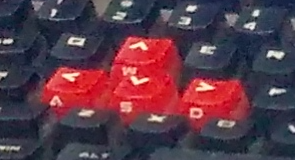
\includegraphics[scale=0.5]{debug/input1}}
		}
		\label{fig:inputFigureSub}
	}
	\quad
	\subfloat[Cluttered environment (\textbf{p2-2-1})]{
		{
			\setlength{\fboxsep}{1pt}
			\setlength{\fboxrule}{1pt}
			\fbox{\includegraphics[scale=0.08]{debug/input2}}
		}
		\label{fig:inputFigureClut}
	}
	\caption{Initial images used on the experiments.}
	\label{fig:inputFigure}
\end{figure}

\textbf{\LARGE Question 3 - Video Stabilization Algorithm}\\

\textbf{3.1 )}\\
Rascunhos a serem ignorados:
* SIFT possui basicamente duas opera��es independentes: detec��o de interest points, chamados de keypoints no artigo e a extra��o de um descritor relacionado a cada keypoint.


\begin{figure}[!h]
	\centering
	\subfloat[Keypoints in sub image (\textbf{p2-3-1-X})]{
		{
			\setlength{\fboxsep}{1pt}
			\setlength{\fboxrule}{1pt}
			\fbox{\includegraphics[scale=0.5]{debug/Keypoints1}}
		}
		\label{fig:keypointsSub}
	}
	\quad
	\subfloat[Keypoints in cluttered image (\textbf{p2-3-1-X})]{
		{
			\setlength{\fboxsep}{1pt}
			\setlength{\fboxrule}{1pt}
			\fbox{\includegraphics[scale=0.08]{debug/KeyPoints2}}
		}
		\label{fig:keypointsClut}
	}
	\caption{Keypoints found by SIFT algorithm.}
	\label{fig:keypoints}
\end{figure}

\textbf{3.2 )} At this point the SIFT transform has given back all the keypoints it has found in both images, as seen in Figure \ref{fig:keypoints}, and all the descriptors also found in both images. But still there is no relation between the keypoints in Figure \ref{fig:keypointsSub} and the ones in Figure \ref{fig:keypointsClut}, and to relate those keypoints a matching process is performed.
\par
	The goal of the matching is to find the same descriptor, or the closest ones, in both Figure \ref{fig:keypointsSub} and Figure \ref{fig:keypointsClut}. To do so an euclidian distance is calculated between any two descriptors, one in each image, and if they are the same then the distance result will be minimal. The distance is calculated between every descriptor in Figure \ref{fig:keypointsSub} and every descriptor in Figure \ref{fig:keypointsClut}. This algorithm isn't perfect and some false positives arise, to eliminate these incorrect relations a new filtering occurs, additional to the closest descriptor match, the second closest descriptor is also retrieved and a ratio between both is calculated, if the ratio between both is greater than 0.75 the relation is ignored. In his article LOWE,2004 suggests a ratio of 0.8 but it didn't performed well with our data.

\begin{figure}[!h]
	\centering
	\subfloat[Ratio of 0.75 (\textbf{p2-3-2-2})]{
		{
			\setlength{\fboxsep}{1pt}
			\setlength{\fboxrule}{1pt}
			\fbox{\includegraphics[scale=0.1]{debug/matches_with_ratio_0_75}}
		}
		\label{fig:ratio75}
	}
	\quad
	\subfloat[Ratio of 0.90 (\textbf{p2-3-2-3})]{
		{
			\setlength{\fboxsep}{1pt}
			\setlength{\fboxrule}{1pt}
			\fbox{\includegraphics[scale=0.1]{debug/matches_with_ratio_0_90}}
		}
		\label{fig:ratio90}
	}
	\caption{Ratio between descriptors distance experiments.}
	\label{fig:matchRatio}
\end{figure}

	Figure \ref{fig:matchRatio} appends Figures \ref{fig:keypointsSub} and Figure \ref{fig:keypointsClut} side by side and uses a OpenCV function (drawMatchesKnn) to connect the matched points. Figure \ref{fig:ratio90} shows that at ratio 0.9 the filter still allows some false positives to go through, and Figure \ref{fig:ratio75} at ratio 0.75 was the best result we had before the filter started cutting out true positives matches, according to LOWE,2004 a ratio of 0.8 should eliminate 90\% of false matches and discard only 5\% of correct matches. We also performed a sandbox experiment, Figure \ref{fig:noRatio} ignoring ratios completely, as expected there are many false positives matches because of these points neighborhoods.
\par
	We believe that our results difference with Lowe's are caused by distinct cameras and scenes.\\

\begin{figure}[!h]
	\centering
		{
			\setlength{\fboxsep}{1pt}
			\setlength{\fboxrule}{1pt}
			\fbox{\includegraphics[scale=0.1]{debug/matches_without_ratio}}
		}
	\caption{Matching process ignoring ratios.}
	\label{fig:noRatio}
\end{figure}

\textbf{3.3 )}
\\
\textbf{3.4 )}
\\

\end{document}
